The class \textit{VM} shown in \refFig{tra_vm_OZ} is mapped to a \picalc{} process \textit{VM\_OZ} shown in \refLis{tra_vm_OZ_listing}. The processes \textbf{VM\_OZ} has sex parameters
\begin{itemize}
\item \textit{self,cv,tv,m}: represents the state variables.
\item \textit{coffee,tea,talk}: represents the operations.
\end{itemize}
The processes \textit{VM\_OZ} mimics the behaviour of $VM$. :
\begin{itemize}
\item on reviving a signal via \textit{coffee} it checks if \textit{VM\_Condition\_IF\_Else\_coffee} the condition \textit{VM\_Condition\_coffee} is fulfilled, then it makes a state transition \textit{VM\_State\_Transition\_coffee} to  decreases \textit{One(b) }| \textit{Sub(cv,b,c,done)} the value of \textit{cv} by one.
\item the same for \textit{tea}.
\item it can send a copy of the value of $self,m$ via $talk$
\end{itemize}

\begin{figure}[H]
\begin{subfigure}{.6\textwidth}
\centering
\begin{class}{VM(id: \integer)}
\\
\begin{state}
cv, tv, m, self: \integer
\ST
0 \leq  cv \leq 3
\\
0 \leq  tv \leq 3
\end{state} 
\\
\begin{init}
cv = 3
\\tv = 3
\\ m= 1
\\self = id
\end{init} 
\\
\begin{op}{coffee}
\Delta (cv)
\ST
cv' = cv - 1
\end{op}
\\
\begin{op}{tea}
\Delta (tv)
\ST
tv' = tv - 1
\end{op}
\\
\begin{op}{talk}
y!: \integer
\\z!: \integer
\ST
y! = m
\\z! = self
\end{op}
\end{class}
  \caption{VM OZ class}
\end{subfigure}%
\begin{subfigure}{.4\textwidth}
  \centering
\fbox{  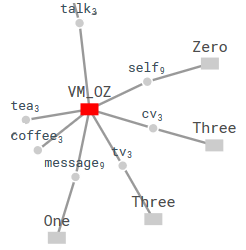
\includegraphics[width=.91\linewidth]{./images/transformational_semantics_of_oz/vm_OZ.png}}
  \caption{stargazer visualization}
\end{subfigure}
\caption{transforming VM into \picalc{} process \textit{VM\_OZ}}
\label{tra_vm_OZ}
\end{figure}

\lstinputlisting[backgroundcolor=\color{white},caption={ VM OZ class as a process in ABC code.},captionpos=b, label={tra_vm_OZ_listing}]{listings/vm_OZ.abc}